% % % % % % % % % % % % % % % % % % % % % % % 
% DOCUMENT SETUP
% % % % % % % % % % % % % % % % % % % % % % % 
\documentclass[12pt]{article}
\usepackage[letterpaper,left=0.75in,right=0.75in,top=1.0in,bottom=1.0in]{geometry}


% % % % % % % % % % % % % % % % % % % % % % % 
% IMPORTED PACKAGES
% % % % % % % % % % % % % % % % % % % % % % % 
\usepackage[utf8]{inputenc}
\usepackage{enumitem}
\usepackage{dsfont}
\usepackage{ulem}
\usepackage{hyperref}
\hypersetup{
    colorlinks=true,
    linkcolor=black,
    urlcolor=blue, 
    breaklinks=true
}
\usepackage{breakcites}
%\usepackage{caption}
\usepackage[version=4]{mhchem}
\usepackage{float}
\usepackage[hang]{subfigure}
\usepackage{overpic}
\usepackage{listings}
\usepackage[super]{nth}
\usepackage{multicol}
\linespread{1.15}
\usepackage{siunitx}
\usepackage{makecell}
\usepackage{booktabs}

% % % % % % % % % % % % % % % % % % % % % % % 
% PROJECT SPECIFICATIONS
% % % % % % % % % % % % % % % % % % % % % % %  
\title{Support Information: \\
Nickel(II) and Copper(II) Supported Metal Complex Stability in NU-1000 Under Hydrogenation Conditions}
\author{Stephen Vicchio}

% % % % % % % % % % % % % % % % % % % % % % % 
% THE DOCUMENT
% % % % % % % % % % % % % % % % % % % % % % %
\begin{document}
\maketitle

\newpage
\tableofcontents

\newpage
\section{Computational Methodology}
\subsection{Deriving Free Energy Expression}
We transformed the free energy from a fixed number of atoms to a fixed chemical potential to account for the compositional variation of the different activated clusters (shown in Equation \ref{eq:transformation1}):
\begin{equation}
    F^{0}(T,P,N_{H},N_{OH},N_{M^{*}}) \rightarrow F^{3}(T,P,\mu_{H^{*}},\mu_{OH^{*}},\mu_{M^{*}})
    \label{eq:transformation1}
\end{equation}
where $N_{H}$ is the number of adsorbed $H$ on the cluster with chemical potential $\mu_{H^{*}}$, $N_{OH}$ is the number of adsorbed $OH$ on the cluster with chemical potential $\mu_{OH^{*}}$, and $N_{M}$ is the number of adsorbed metal species ($M$) on the cluster with chemical potential $\mu_{M^{*}}$. Using Legendre's transforms, the free energy is is written as Equation \ref{eq:transformation2}:
\begin{equation}
    \begin{split}
        F^{3}(T,P,\mu_{H^{*}},\mu_{OH^{*}},\mu_{M^{*}}) &= F^{0}(T,P,N_{H},N_{OH},N_{M^{*}}) \\ &- (\mu_{H^{*}})(N_{H}) \\ &- (\mu_{OH^{*}})(N_{OH}) \\ &- (\mu_{M^{*}})(N_{M^{*}})  
        \label{eq:transformation2}    
    \end{split}
\end{equation}
The new free energy expression (Equation \ref{eq:transformation2}) allows for compositionally different structures to be compared with the gas phase conditions being included in the free energy expression. The final free energy expression defining the difference between the modified ($k$) and the reference ($i$) structure is defined in Equation \ref{eq:freenergyfinal}:
\begin{equation}
    \begin{split}
        \Delta F^{(3)}(T,\mu_{H^{*}},\mu_{OH^{*}},\mu_{M^{*}})  = 
        & F_{j}(T,N_{j,H^{*}},N_{j,OH^{*}},N_{j,M^{*}}) - 
          F_{i}(T,N_{i,H^{*}},N_{i,OH^{*}},N_{i,M^{*}}) \\
        & - (\mu_{H^{*}})(\Delta N_{H^{*}}) - (\mu_{OH^{*}})(\Delta N_{OH^{*}}) - (\mu_{M^{*}})(\Delta N_{M^{*}}) \\ 
    \end{split}
    \label{eq:freenergyfinal}
\end{equation}
where $\Delta N_{i}$ terms represent the different between the modified ($N_{j}$) and reference ($N_{i}$) structures for a particular species. The $^{*}$ indicates the species is bound to the cluster. For both models (\ce{Cu} and \ce{Ni}), the model is comprised of \ce{OH} ligands linking the metal atoms and connecting the \ce{Zr} nodes. To relate the free energy to reaction conditions ($T$ and $P$), the adsorbed species chemical potential must be related to the chemical potential of the gas phase species through equilibrium expressions. \\ 

\subsubsection{Equilibrium expression for $H^{*}$}
For $H^{*}$, the assumed equilibrium is with a reservoir of \ce{H2} gas:
\begin{equation}
    \frac{1}{2} H_{2} \ce{<=>} H^{*}
\end{equation}
where the chemical potential terms are related by: 
\begin{equation}
    \frac{1}{2} \mu_{H_{2}}^{g}(T,P) = \mu_{H^{*}}
\end{equation}  
The $\mu_{H_{2}}^{g}(T,P)$ is computed by  correcting the electronic energy (referenced at $T$=0 K) of an isolated molecule with the gas-phase Gibbs free energy values at a specific temperature and pressure (shown in Equation \ref{H2-to-reaction-conditions}). 
\begin{equation}
    \begin{split}
         \mu_{H_{2}}^{g}(T,P) &= E_{H_{2}}^{DFT} + E_{H_{2}}^{ZPE} + \Delta \mu_{H_{2}}(T,P)  \\
         \mu_{H_{2}}^{g}(T,P) &= E_{H_{2}}^{DFT} + E_{H_{2}}^{ZPE} + \Delta G_{H_{2}}(T,P) \\ 
         \mu_{H_{2}}^{g}(T,P) &= E_{H_{2}}^{DFT} + E_{H_{2}}^{ZPE} + \Big[ \Delta G_{H_{2}}(T,P^{o})  + RT \ln{ \frac{P_{H_2}}{P_{H_2}^{o}}} \Big]  \\ 
    \end{split}
    \label{H2-to-reaction-conditions}
\end{equation}
With all calculations being performed at 0 K, the $G_{H_{2}}(T,P)$ was referenced to 0 K when evaluating the free energy from pMuTT. The electronic energy ($E_{H_{2}}^{DFT}$) and zero-point energy ($E_{H_{2}}^{ZPE}$) were calculated in CP2K using the same computational parameters as described in the methodology section of the manuscript. 

\subsubsection{Equilibrium expression for $OH^{*}$}
For $OH^{*}$, the assumed equilibrium is with a reservoir of \ce{H2} and \ce{H2O} gas:
\begin{equation}
    \frac{1}{2} H_{2} + OH \ce{<=>} H_{2}O
\end{equation}
where the chemical potential terms are related by: 
\begin{equation}
    \frac{1}{2} \mu_{H_{2}^{g}}(T,P) + \mu_{OH^{*}} = \mu_{H_{2}O}^{g}(T,P) 
\end{equation}
The \ce{OH^{*}} chemical potential term is dependent on both the \ce{H2} and \ce{H2O} gas phase conditions. 
\begin{equation}
    \mu_{OH^{*}} = \mu_{H_{2}O}(T,P) - \frac{1}{2} \mu_{H_{2}}(T,P)    
\end{equation}
The $\mu_{H_{2}O}^{g}(T,P)$ was evaluated just like $\mu_{H_{2}}^{g}(T,P)$ in Equation \ref{H2-to-reaction-conditions}. 
\begin{equation}
    \begin{split}
         \mu_{H_{2}O}^{g}(T,P) &= E_{H_{2}O}^{DFT} + E_{H_{2}O}^{ZPE} + \Delta \mu_{H_{2}O}(T,P)  \\
         \mu_{H_{2}O}^{g}(T,P) &= E_{H_{2}O}^{DFT} + E_{H_{2}O}^{ZPE} + \Delta G_{H_{2}O}(T,P) \\ 
         \mu_{H_{2}O}^{g}(T,P) &= E_{H_{2}O}^{DFT} + E_{H_{2}O}^{ZPE} + \Big[ \Delta G_{H_{2}O}(T,P)  + RT \ln{ \frac{P_{H_{2}O}}{P_{H_{2}O}^{o}}} \Big]  \\ 
    \end{split}
    \label{H2O-to-reaction-conditions}
\end{equation}
With all calculations being performed at 0 K, the $G_{H_{2}}(T,P)$ was referenced to 0 K when evaluating the free energy from pMuTT. The combined expression for $\mu_{OH^{*}}$ is given by Equation \ref{OH-to-reaction-conditions}.
\begin{equation}
    \begin{split}
    \mu_{OH^{*}} &=  E_{H_{2}O}^{DFT} + E_{H_{2}O}^{ZPE} + \Big[ \Delta G_{H_{2}O}(T,P^{o})  + RT \ln{ \frac{P_{H_{2}O}}{P_{H_{2}O}^{o}}} \Big] \\
    &- \frac{1}{2} \Big[ E_{H_{2}}^{DFT} + E_{H_{2}}^{ZPE} + \big[ \Delta G_{H_{2}}(T,P^{o})  + RT \ln{ \frac{P_{H_2}}{P_{H_2}^{o}}} \big] \Big] 
    \end{split}
    \label{OH-to-reaction-conditions}
\end{equation} 
The $\mu_{OH^{*}}$ chemical potential is dependent on temperature ($T$) and both gas phase partial pressures ($P_{H_2}$ and $P_{H_{2}O}$). The electronic energy ($E_{H_{2}O}^{DFT}$) and zero-point energy ($E_{H_{2}O}^{ZPE}$) were calculated in CP2K using the same computational parameters as described in the methodology section of the manuscript. \\

\subsubsection{Equilibrium expression for $M^{*}$}
For $M^{*}$, the assumed equilibrium is with a reservoir of bulk-\ce{M}:
\begin{equation}
    bulk-M \ce{<=>} M^{*}
\end{equation}
where the chemical potential terms are related by: 
\begin{equation}
    \mu_{bulk-M} = \mu_{M^{*}}
\end{equation}
Unlike $\mu_{OH^{*}}$ and $\mu_{H^{*}}$, $\mu_{M^{*}}$ was determined by the  electronic energy of a bulk metal surface (Equation \ref{Ni-to-reaction-conditions})
\begin{equation}
    \mu_{M^{*}} = \mu_{bulk-M} = E_{M}^{DFT}
    \label{Ni-to-reaction-conditions}
\end{equation}
%TODO explain that the computational parameters are different here.... 

\subsection{Final Transformed Free Energy Expression}
The final transformed free energy expression is given by Equation \ref{eq:final-free-energy-equation-full}. All the terms dervied above are included in the expression. 
\begin{equation}
    \begin{split}
        \Delta F^{(3)}(T,\mu_{H^{*}},\mu_{OH^{*}},\mu_{M^{*}})  = 
        & F_{j}(T,N_{j,H^{*}},N_{j,OH^{*}},N_{j,M^{*}}) - 
          F_{i}(T,N_{i,H^{*}},N_{i,OH^{*}},N_{i,M^{*}}) \\
        & - (\Delta N_{H^{*}}) (E_{H_{2}}^{DFT} + E_{H_{2}}^{ZPE} + \Big[ \Delta G_{H_{2}}(T,P^{o})  + RT \ln{ \frac{P_{H_2}}{P_{H_2}^{o}}} \Big])  \\
        & - (\Delta N_{OH^{*}}) \Big( E_{H_{2}O}^{DFT} + E_{H_{2}O}^{ZPE} + \Big[ \Delta G_{H_{2}O}(T,P^{o})  + RT \ln{ \frac{P_{H_{2}O}}{P_{H_{2}O}^{o}}} \Big] \\ 
        & - \frac{1}{2} \Big[ E_{H_{2}}^{DFT} + E_{H_{2}}^{ZPE} + \big[ \Delta G_{H_{2}}(T,P^{o})  + RT \ln{ \frac{P_{H_2}}{P_{H_2}^{o}}} \big] \Big] \Big) \\
        & - (\Delta N_{M^{*}}) (E_{M}^{DFT}) \\ 
    \end{split}
    \label{eq:final-free-energy-equation-full}
\end{equation}

\newpage
\subsection{pMuTT Expressions}

\subsubsection{Gas Phase Free Energy as a Function of Temperature}
The NASA Polynomials are defined for a very specific temperature range. To correct the electronic energies from DFT, the gas phase species must be referenced to approximately 0 K. When using pMuTT, the reference state for the free energy values is $298 K$. The empirical methods do not allow for referencing at 0 K, so the free energies are approximated by values at 10 K (shown below):

\begin{equation}
    \begin{split}
        \Delta G(T) &= [G(T) - G(T=298 K)] - [G(T=10 K) - G(T=298 K)] \\
        \Delta G(T) &= [G(T)] - [G(T=10 K)] 
    \end{split}
\end{equation} 
where $\Delta G(T)$ is the free energy referenced at $T = 10 K$, and G(T) is the free energy reference at $T = 298 K$. 

\begin{figure}[H]
    \centering
    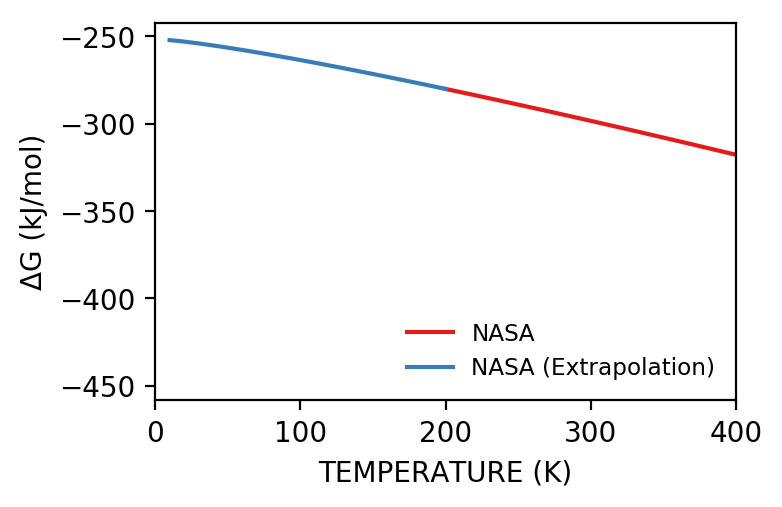
\includegraphics[width=0.70\textwidth]{zi-images/00-General-Graphics/2021-figure-H2-pMuTT.png}
    \caption{The gas phase free energy of \ce{H2} as a function of temperature. The reference state it defined as 10 K. The red line shows the NASA Polynomial within defined range, and the blue line shows the extrapolation.}
    \label{fig:h2-pmutt-expression}
\end{figure}

\begin{figure}[H]
    \centering
    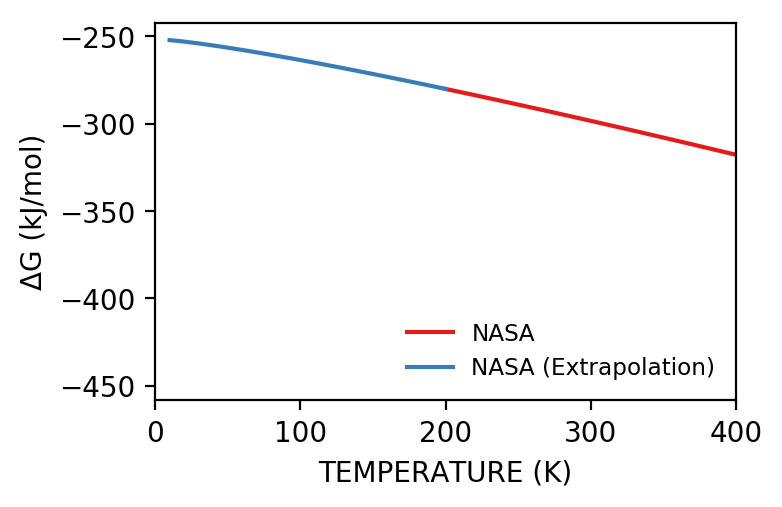
\includegraphics[width=0.70\textwidth]{zi-images/00-General-Graphics/2021-figure-H2O-pMuTT.png}
    \caption{The gas phase free energy of \ce{H2O} as a function of temperature. The reference state it defined as 10 K. The red line shows the NASA Polynomial within defined range, and the blue line shows the extrapolation.}    \label{fig:h2o-pmutt-expression}
\end{figure}

%TODO do I need a statement here about the bulk model and where the bulk models ended up coming from?



\subsection{Spin Contamination}
The library was optimized at different \ce{Ni} spin states; the considered spin states for \ce{Ni(II)} were singlet (no unpaired electrons) and triplet (two unpaired electrons). With the cluster initially containing four \ce{Ni(II)} species, the intermediate combinations were calculated (one singlet and three triplet, two singlet and two triplet, etc.). Structures that exhibited spin contamination were removed from the analysis. Comparisons between the ideal and single determinant $S^{**}2$ values were inspected. If the single determinant value deviated by more than 10\% of the ideal determinant the structure was removed from analysis. 
\begin{center}
\begin{table}[H]
\centering
  \setlength\tabcolsep{8pt}
  \caption{Example of Spin Contamination Analysis for \ce{Ni4(OH)6 \cdot 2H} Structure.}
  \label{tbl:spin_contamination}
  \begin{tabular}{lcccc}
    \hline
        \ce{Ni(II)} Spin Configuration  & \thead{ Electronic \\ Energy (hartree)} &  Ideal $S^{**}2$ &   Single $S^{**}2$ & Contamination? \\
        \hline
        a) Four singlet (RKS\textsuperscript{a}) & -4778.84071 & N\/a & N\/a & No \\
        b) Four singlet (UKS)                    & -4778.87973 & 0.000  & 2.386  & Yes \\
        c) Three singlet, one triplet            & -4778.88313 & 2.000  & 3.978  & Yes \\
        d) Two singlet, two triplet              & -4778.88042 & 6.000  & 6.457  & Yes \\
        e) One singlet, three triplet            & -4778.88209 & 12.000 & 12.014 & No \\
        f) Four triplet                          & -4778.84120 & 20.000 & 20.013 & No \\
        \hline
    \end{tabular} \\
    \textsuperscript{a} Restricted Kohn-Sham \\
\end{table}    
\end{center}
From Table \ref{tbl:spin_contamination}, the lowest energy structure is  c) three singlet, one triplet; however, the structure is removed from the analysis because the ideal $S^{**}2$ and single $S^{**}2$ deviate. Therefore, the lowest energy structure for this particular configuration is the e) one singlet, three triplet. This type of analysis was included for all structures. 

\newpage
\subsection{Sample Input File}
Below is a sample CP2K input file. If the singlet spin state was desired for all \ce{Ni(II)} atoms, UKS F and MULTIPLICITY 1 were used. 
\begin{center}
    \lstset{numbers=left, basicstyle=\ttfamily, numbersep=-45pt}
    \begin{lstlisting}[language=bash]
        &GLOBAL
           PRINT_LEVEL  MEDIUM
           PROJECT_NAME info-ni4oh6-4h2o-config2-MULTI9
           RUN_TYPE  GEO_OPT
           WALLTIME 71:47:00
         &END GLOBAL
         &MOTION
           &GEO_OPT
             TYPE  MINIMIZATION
             OPTIMIZER  BFGS
             MAX_ITER  2000
             MAX_DR     5.0000000000000001E-04
             MAX_FORCE     5.0000000000000002E-05
             RMS_DR     5.0000000000000001E-04
             RMS_FORCE     5.0000000000000002E-05
             STEP_START_VAL  603
             &BFGS
               TRUST_RADIUS     2.5000000000000006E-01
             &END BFGS
           &END GEO_OPT
         &END MOTION
         &FORCE_EVAL
           METHOD  QS
           STRESS_TENSOR  ANALYTICAL
           &DFT
             BASIS_SET_FILE_NAME BASIS_file
             POTENTIAL_FILE_NAME POTENTIALS_file
             UKS  T
             MULTIPLICITY  9
             CHARGE  0
             &SCF
               MAX_SCF  1000
               EPS_SCF     9.9999999999999995E-07
               SCF_GUESS  ATOMIC
               &OT  T
                 MINIMIZER  CG
                 PRECONDITIONER  FULL_ALL
                 ENERGY_GAP     1.0000000000000000E-03
               &END OT
               &OUTER_SCF  T
                 EPS_SCF     9.9999999999999995E-07
                 MAX_SCF  50
               &END OUTER_SCF
             &END SCF
             &QS
               EPS_DEFAULT     1.0000000000000000E-10
               METHOD  GPW
             &END QS
             &MGRID
               NGRIDS  5
               CUTOFF     3.6000000000000000E+02
               REL_CUTOFF     8.0000000000000000E+01
             &END MGRID
             &XC
               DENSITY_CUTOFF     1.0000000000000000E-10
               GRADIENT_CUTOFF     1.0000000000000000E-10
               TAU_CUTOFF     1.0000000000000000E-10
               &XC_FUNCTIONAL  NO_SHORTCUT
                 &PBE  T
                 &END PBE
               &END XC_FUNCTIONAL
               &VDW_POTENTIAL
                 POTENTIAL_TYPE  PAIR_POTENTIAL
                 &PAIR_POTENTIAL
                   TYPE  DFTD3(BJ)
                   PARAMETER_FILE_NAME dftd3.dat
                   REFERENCE_FUNCTIONAL PBE
                   CALCULATE_C9_TERM  F
                 &END PAIR_POTENTIAL
               &END VDW_POTENTIAL
             &END XC
           &END DFT
           &SUBSYS
             &CELL
               A     4.061108E+01   0.00000E+00    0.00000E+00
               B     2.03054E+01    3.51702E+01    0.00000E+00
               C     0.00000E+00    0.00000E+00    1.59897E+01
               MULTIPLE_UNIT_CELL  1 1 1
               SYMMETRY  MONOCLINIC_GAMMA_AB
             &END CELL
             &KIND C
               BASIS_SET DZVP-MOLOPT-SR-GTH-q4
               POTENTIAL GTH-PBE-q4
             &END KIND
             &KIND H
               BASIS_SET DZVP-MOLOPT-SR-GTH-q1
               POTENTIAL GTH-PBE-q1
             &END KIND
             &KIND Ni
               BASIS_SET DZVP-MOLOPT-SR-GTH-q18
               POTENTIAL GTH-PBE-q18
             &END KIND
             &KIND O
               BASIS_SET DZVP-MOLOPT-SR-GTH-q6
               POTENTIAL GTH-PBE-q6
             &END KIND
             &KIND Zr
               BASIS_SET DZVP-MOLOPT-SR-GTH-q12
               POTENTIAL GTH-PBE-q12
             &END KIND
             &TOPOLOGY
               COORD_FILE_NAME ./sNi4OH6-4H2O-config2.xyz
               COORD_FILE_FORMAT  XYZ
               NUMBER_OF_ATOMS  584
               CONN_FILE_FORMAT  OFF
               MULTIPLE_UNIT_CELL  1 1 1
             &END TOPOLOGY
           &END SUBSYS
           &PRINT
             &FORCES  ON
             &END FORCES
           &END PRINT
         &END FORCE_EVAL
    \end{lstlisting}
\end{center}

\newpage
\section{Water Content Phase Diagram}
\begin{figure}[H]
   \centering
    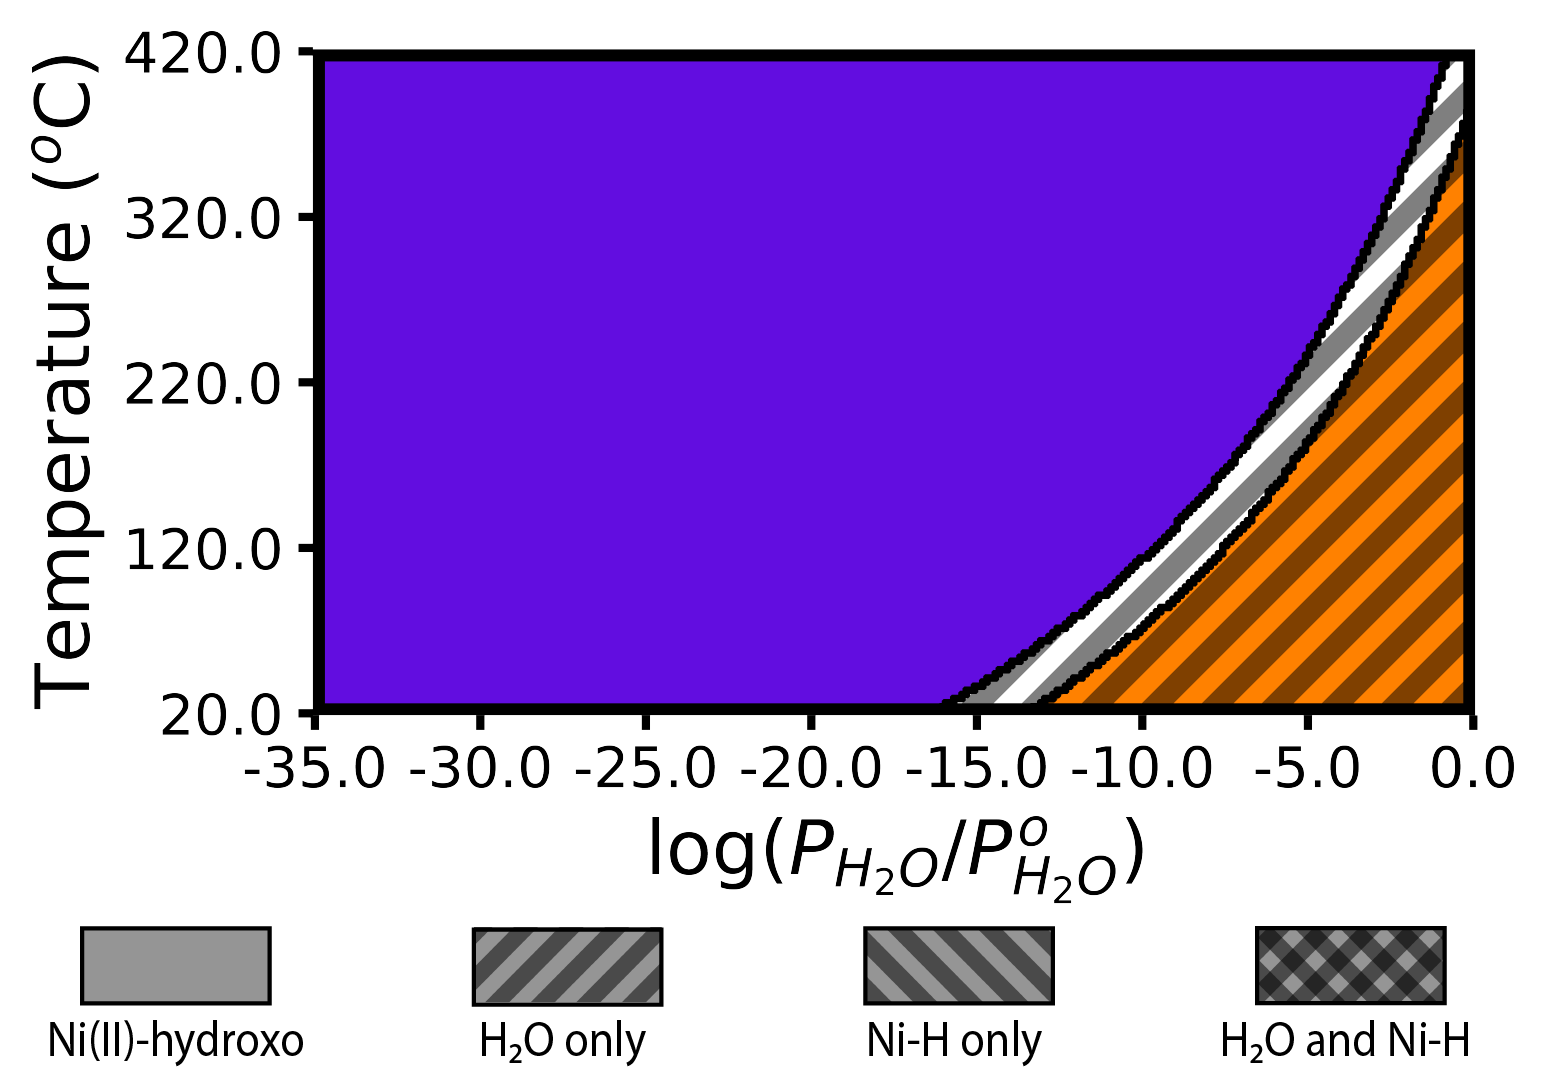
\includegraphics{zi-images/00-General-Graphics/2021-figure-H2O-phase-diagram-manuscript.png}
   \caption{}
   \label{fig:phase-diagram-h2o}
\end{figure}

\section{Generating Phase Diagram structures with inter-atomic distances}

\end{document}